\chapter{Inicialización}

\section{Planificación General}
El presente proyecto esta planteado para ser desarrollado en 20 dias

\section{Identificación de Requerimientos}
\subsection{Requerimientos del sistema}
\begin{table}[H]
    \caption{Tabla de planificación de las diferentes fases del modelo Cascada}
    \label{tabla:ejemplo}
    \begin{center}
        \begin{tabular}{|c|l|c|c|c|}
            \hline
            \textbf{Num.} & \textbf{Fase}  &  \textbf{Fecha inicial} & \textbf{Fecha final} & \textbf{Duración (días)}\\ \hline
            \textbf{1.} & Fase de requerimientos        & 6-jun        & 17-jun        & 10        \\ \hline
            \textbf{2.} & Fase de diseño del sistema       & 20-jun        & 8-jul        & 15        \\ \hline
            \textbf{3.} & Fase de implementación        & 11-jul        & 19-ago        & 30        \\ \hline
            \textbf{4.} & Fase de pruebas        & 22-ago         &   2-sep     &    10     \\ \hline
            \textbf{5.} & Fase de mantenimiento        & 5-sep        & 9-sep        & 5        \\ \hline
        \end{tabular}
    \end{center}
    \begin{center}
        Fuente: Elaboración propia.
    \end{center}
    % Nota. Extraída de Apellido, N. (2000) \textit{Nombre del libro}.
    % Editorial o universidad que lo publicó.
    
\end{table}


Referenciando a la figura \ref{fig:gannt}.
\begin{figure}[H]
    \begin{center}
        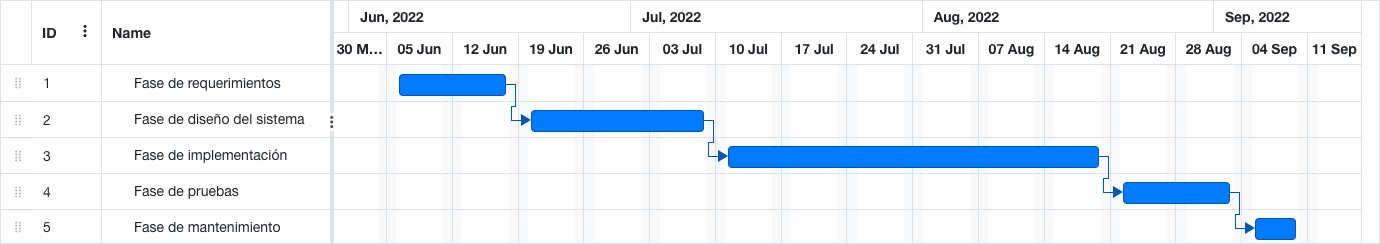
\includegraphics[width=17cm]{img/capitulo_4/gant.png}
        \caption{Diagrama de Gannt.}
        Fuente : Elaboración propia
        \label{fig:gannt}
    \end{center}
\end{figure}

Referenciando a la figura \ref{fig:camera_screen}.
\begin{figure}[H]
    \begin{center}
        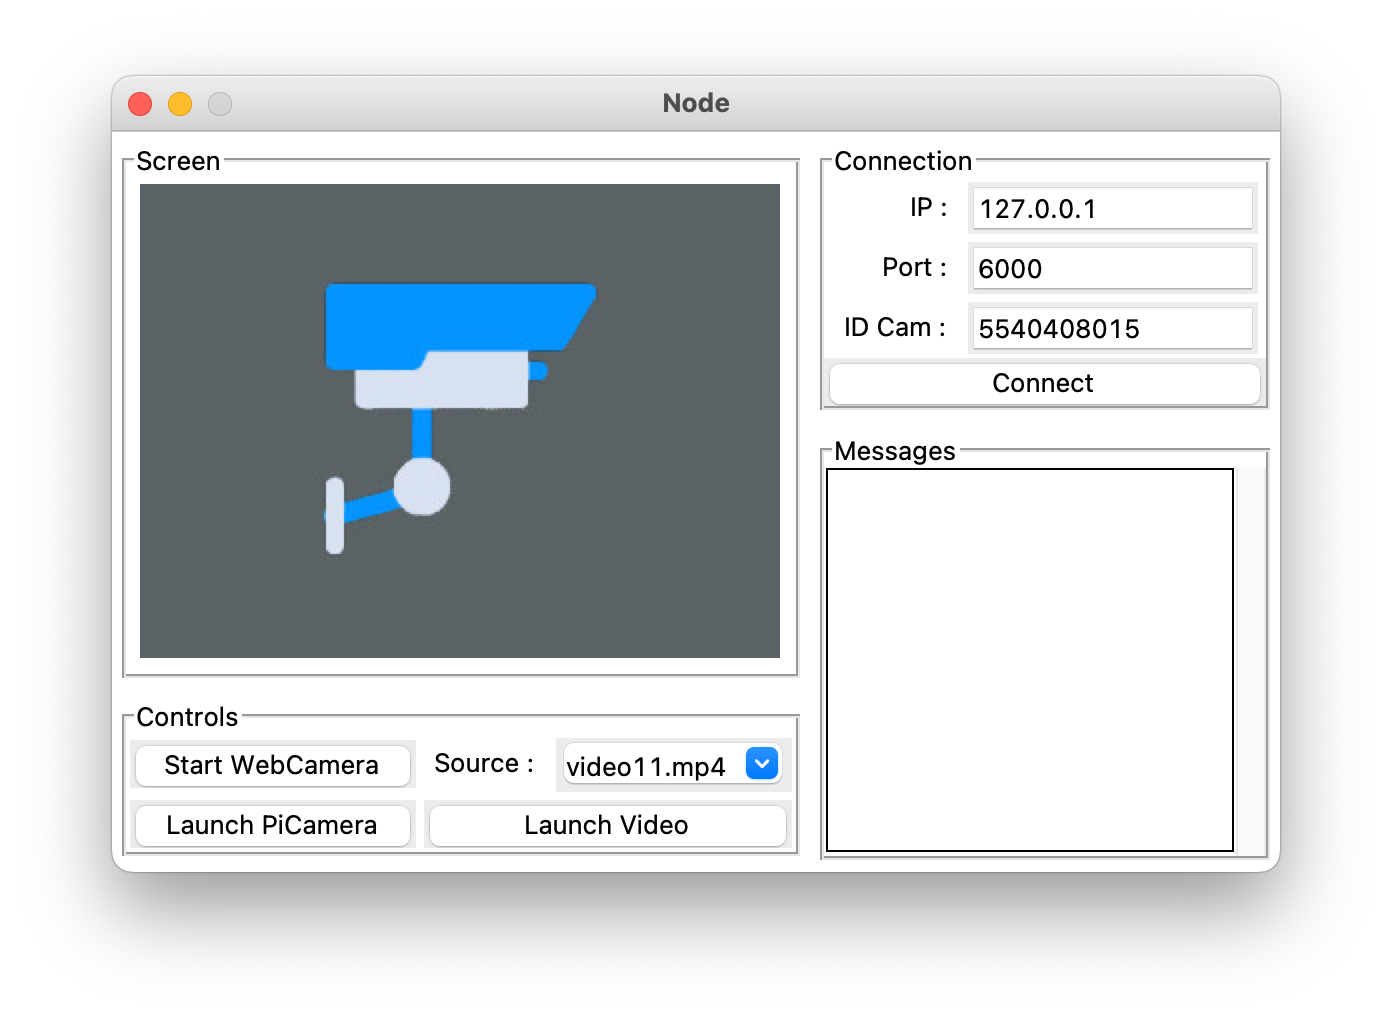
\includegraphics[width=13cm]{img/capitulo_4/camera_screen.png}
        \caption{Diagrama de Gannt.}
        Fuente : Elaboración propia
        \label{fig:camera_screen}
    \end{center}
\end{figure}

Referenciando a la figura \ref{fig:camera_screen}.
\begin{figure}[H]
    \begin{center}
        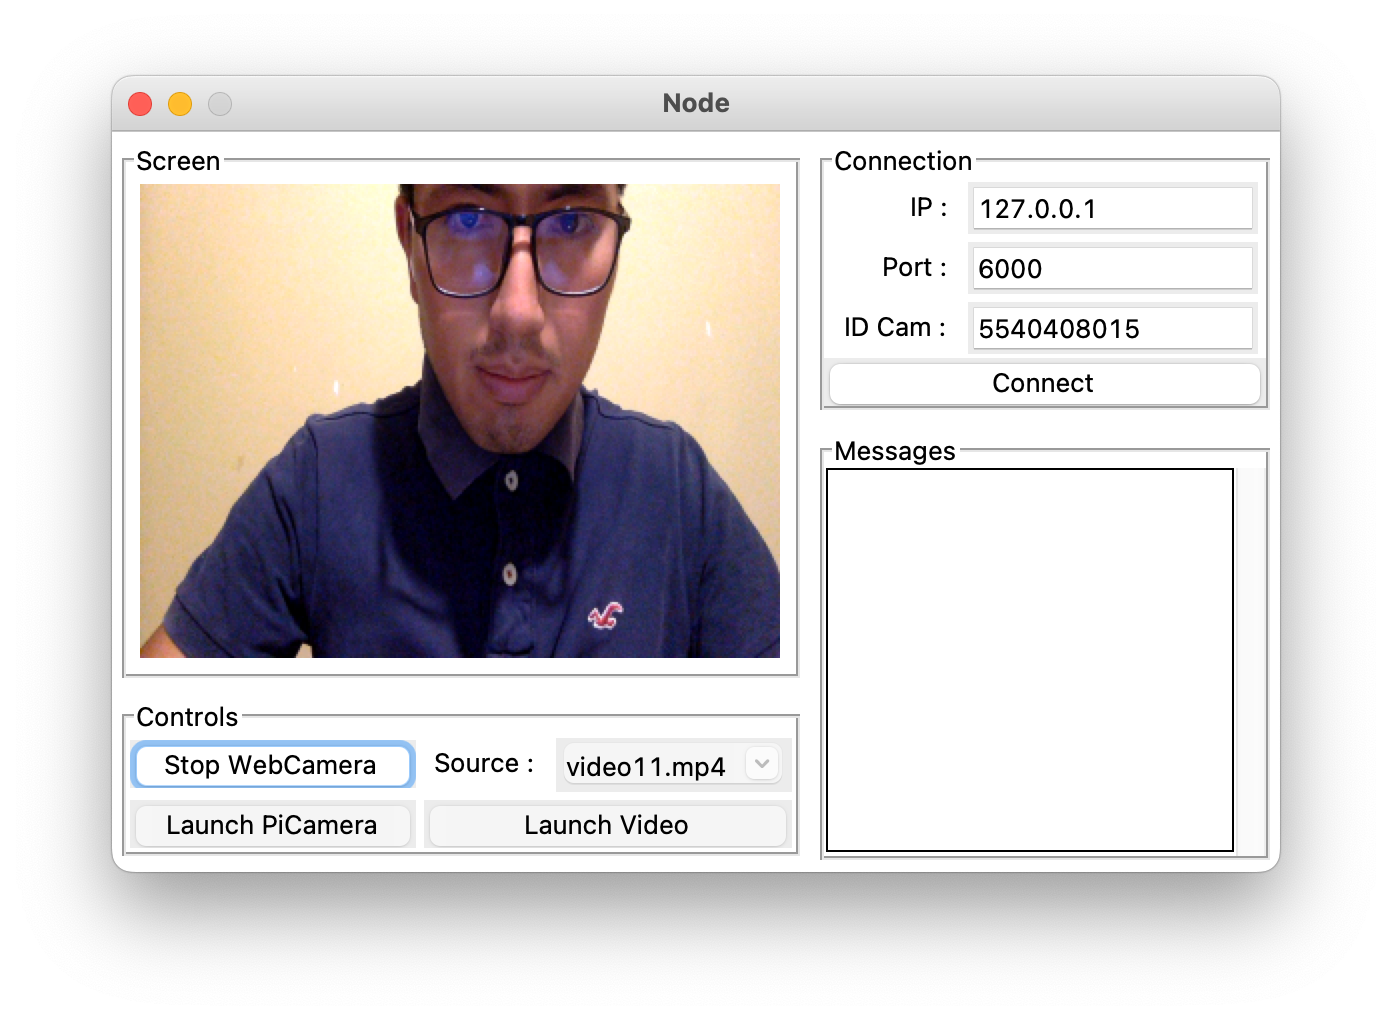
\includegraphics[width=13cm]{img/capitulo_4/webcamera.png}
        \caption{Diagrama de Gannt.}
        Fuente : Elaboración propia
        \label{fig:webcamera}
    \end{center}
\end{figure}

Referenciando a la figura \ref{fig:securityvideo}.
\begin{figure}[H]
    \begin{center}
        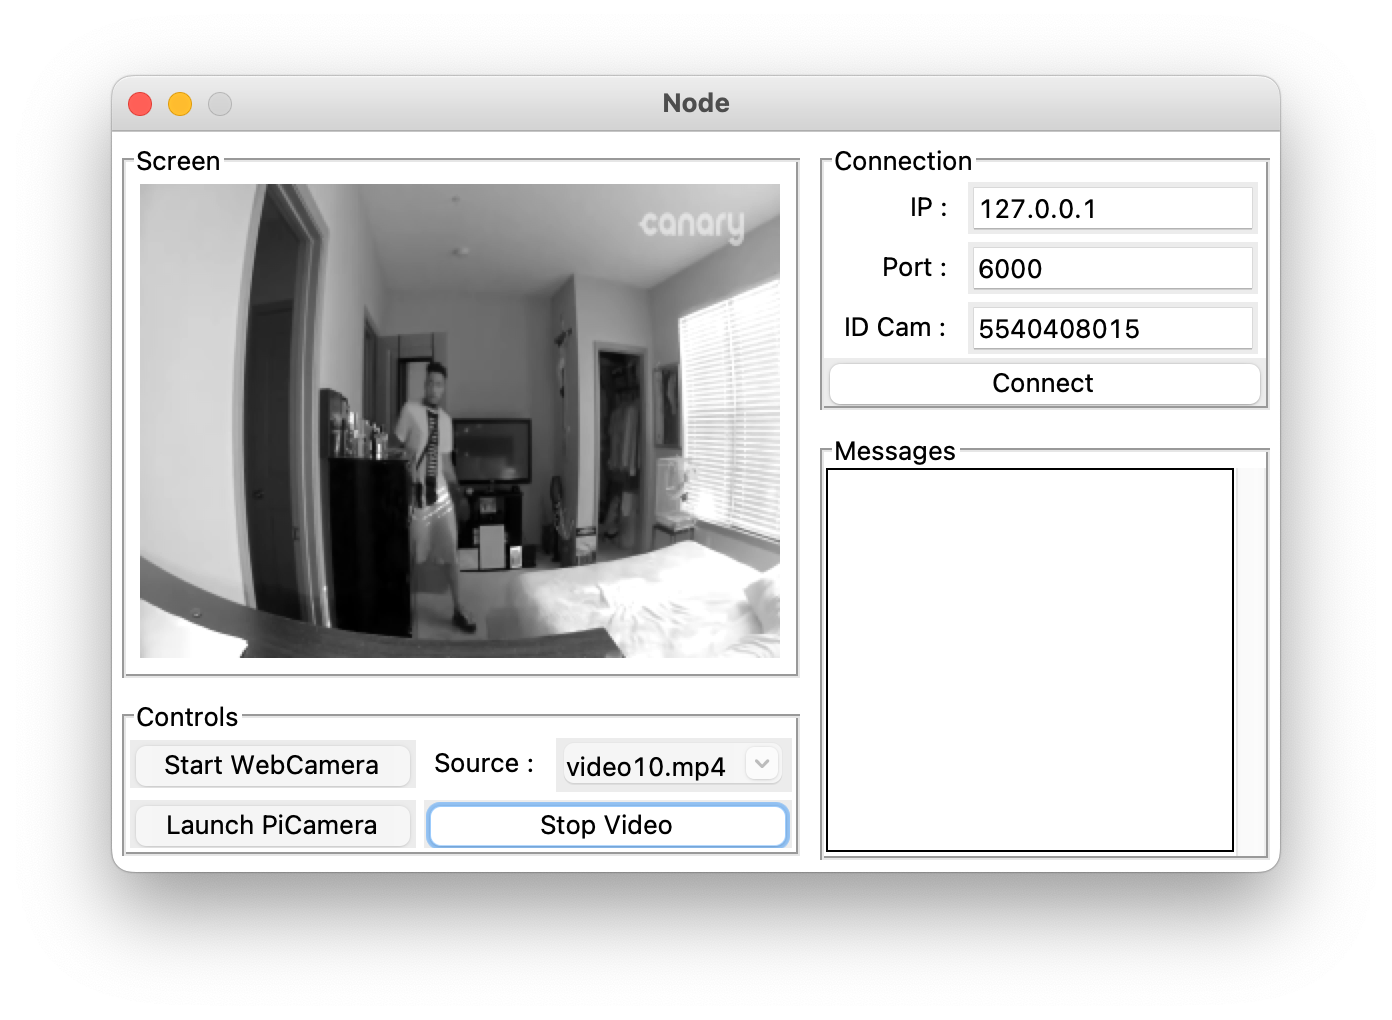
\includegraphics[width=13cm]{img/capitulo_4/security-video.png}
        \caption{Diagrama de Gannt.}
        Fuente : Elaboración propia
        \label{fig:securityvideo}
    \end{center}
\end{figure}

Referenciando a la figura \ref{fig:servertcp_console}.
\begin{figure}[H]
    \begin{center}
        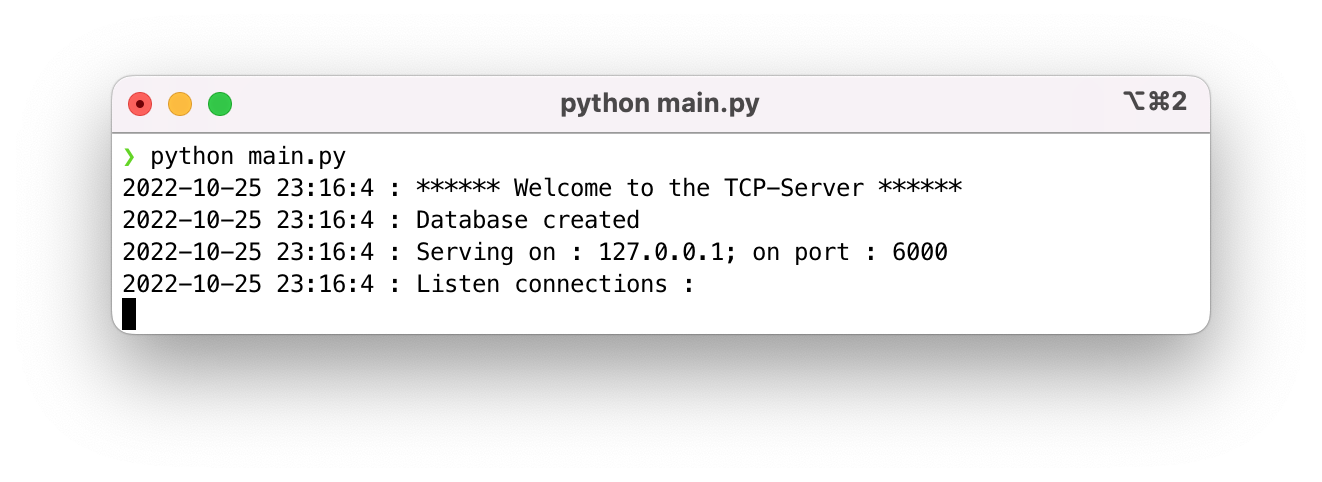
\includegraphics[width=15cm]{img/capitulo_4/tcp_server.png}
        \caption{Ejecución del servidor TCP.}
        Fuente : Elaboración propia
        \label{fig:servertcp_console}
    \end{center}
\end{figure}

\begin{center}
    \begin{tabular}{ |c|c|c|c| } 
    \hline
    \textbf{col1} & \textbf{col2} & \textbf{col3} \\
    \hline
    \multirow{3}{4em}{Multiple row} & cell2 & cell3 \\ 
    & cell5 & cell6  \\
    & cell8 & cell9 \\ 
    \hline
    \end{tabular}
\end{center}

\begin{center}
    \begin{tabular}{ |c|c| } 
     \hline
     1. & Requerimiento uno\\
     \hline 
     2. & Requerimiento dos \\ 
     \hline
     3. & Requerimiento tres \\ 
     \hline
    \end{tabular}
\end{center}

\subsection{Requerimientos del software}

\section{Análisis}
\section{Diseño de Módulos}

\begin{table}[H]
    \caption{Detalle de las pruebas realizadas}
    \label{tabla:ejemplo}
    \begin{center}
        \begin{tabular}{c|c|c|c|}
            \cline{2-4}
            & \textbf{Columna 1} & \textbf{Columna 2} & \textbf{Columna 3} \\ \hline
            \multicolumn{1}{|c|}{\textbf{Fila 1}} & item               & item               & item               \\ \hline
            \multicolumn{1}{|c|}{\textbf{Fila 2}} & item               & item               & item               \\ \hline
            \multicolumn{1}{|c|}{\textbf{Fila 3}} & item               & item               & item               \\ \hline
        \end{tabular}
    \end{center}
    Nota. Extraída de Apellido, N. (2000) \textit{Nombre del libro}.
    Editorial o universidad que lo publicó.
\end{table}

% \usepackage{cellspace}
% \setlength\cellspacetoplimit{4pt}
% \setlength\cellspacebottomlimit{4pt}
% \newcommand\cincludegraphics[2][]{\raisebox{-0.3\height}{\includegraphics[#1]{#2}}}
\begin{table}[H]
    \caption{Detalle de las pruebas realizadas}
    \begin{center}
        \begin{tabular}{|>{\centering}p{0.3\textwidth}|>{\centering}m{0.3\textwidth}|m{0.3\textwidth}<{\centering}|} 
            \hline
            \textbf{Columna 1} & \textbf{Columna 2} & \textbf{Columna 3} \\
            \hline
            \begin{minipage}{.3\textwidth}
                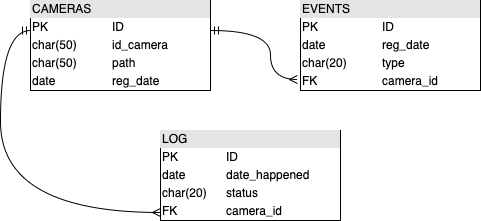
\includegraphics[width=\linewidth]{img/capitulo_4/db.png}
            \end{minipage}& lorem lorem lorem lorem lorem lorem lorem lorem lorem lorem lorem lorem lorem lorem lorem lorem lorem lorem lorem lorem lorem
            & \begin{itemize} 
                \item Remote delivery 
                \item Immersive experiences
                \item text proved
            \end{itemize} \\ 
            \hline
            \begin{minipage}{.3\textwidth}
                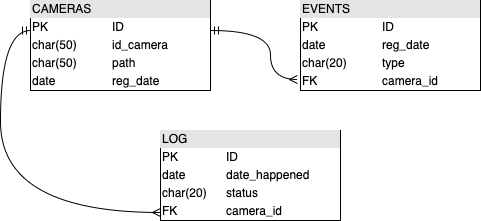
\includegraphics[width=\linewidth]{img/capitulo_4/db.png}
            \end{minipage} & cell8 & \begin{itemize} 
                \item Remote delivery 
                \item Immersive experiences
                \item text proved
            \end{itemize} \\
            \hline
        \end{tabular}
    \end{center}
\end{table}

\begin{table}[H]
    \caption{Detalle de las pruebas realizadas}
    \begin{center}
        \begin{tabular}{|>{\centering}p{0.6\textwidth}|m{0.3\textwidth}<{\centering}|} 
            \hline
            \textbf{Columna 1} & \textbf{Columna 3} \\
            \hline
            \begin{minipage}{.3\textwidth}
                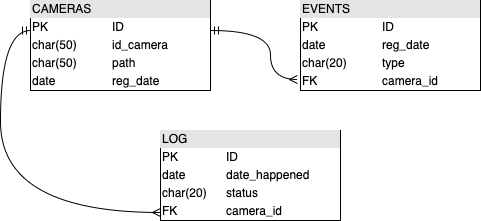
\includegraphics[width=\linewidth, height=40mm]{img/capitulo_4/db.png}
            \end{minipage}
            & \begin{itemize} 
                \item Remote delivery 
                \item Immersive experiences
                \item text proved
            \end{itemize} \\ 
            \hline
            \begin{minipage}{0.6\textwidth}
                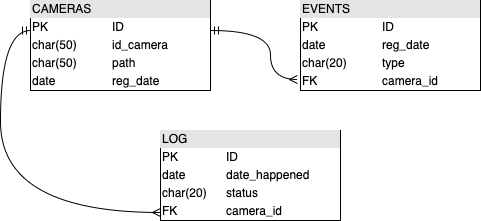
\includegraphics[width=\linewidth]{img/capitulo_4/db.png}
            \end{minipage} & \begin{itemize} 
                \item Remote delivery 
                \item Immersive experiences
                \item text proved
            \end{itemize} \\
            \hline
        \end{tabular}
    \end{center}
\end{table}


\begin{table}[H]
    \caption{Detalle de las pruebas realizadas}
    \label{tabla:ejemplo}
    \begin{center}
        \begin{tabular}{c|c|c|c|}
            \cline{2-4}
            & \textbf{Columna 1} & \textbf{Columna 2} & \textbf{Columna 3} \\ \hline
            \multicolumn{1}{|c|}{Fila 1 }& item             & item               & item               \\ \hline
            \multicolumn{1}{|c|} {Fila 2} & {item}               & item               & item               \\ \hline
            \multicolumn{1}{|c|} {Fila 3} & {item}              & item               & item               \\  \hline
        \end{tabular}
    \end{center}
    Nota. Extraída de Apellido, N. (2000) \textit{Nombre del libro}.
    Editorial o universidad que lo publicó.
\end{table}

\section{Identificación de Subsistemas}

Referenciando a la figura \ref{fig:ejemplo}.
\begin{figure}[H]
    \begin{center}
        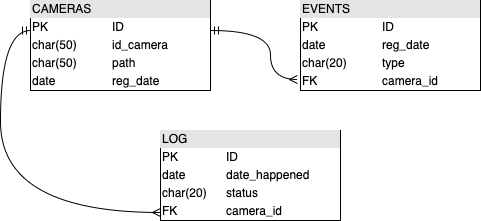
\includegraphics[width=10cm]{img/capitulo_4/db.png}
    \end{center}
    \caption{Ilustración de un ladrón}
    Fuente: Adaptada de Apellido, N. (2000) \textit{Nombre del libro}.
    Editorial o universidad que lo publicó.
    \label{fig:ejemplo}
\end{figure}

Referenciando a la figura \ref{fig:ejemplo}.
\begin{figure}[H]
    \begin{center}
        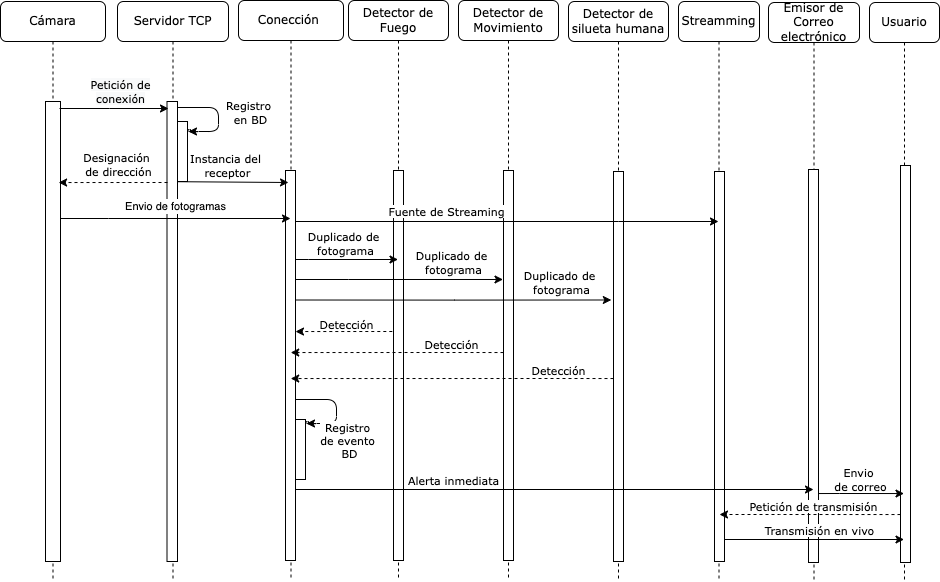
\includegraphics[width=18cm]{img/capitulo_4/interaccion.png}
    \end{center}
    \caption{Ilustración de un ladrón}
    Fuente: Adaptada de Apellido, N. (2000) \textit{Nombre del libro}.
    Editorial o universidad que lo publicó.
    \label{fig:ejemplo}
\end{figure}
\section{Comunicación de Sistemas}

\subsection{Sockets}

\section{Planificación}
